%%%%%%%%%%%%%%%%%%%%%%%%%%%%%%%%%%%%%%%%%%%%%%%%%%%%%%%%%%%%%%%%%%%%%%%%%
%                           Marco Conceptual                               %
%%%%%%%%%%%%%%%%%%%%%%%%%%%%%%%%%%%%%%%%%%%%%%%%%%%%%%%%%%%%%%%%%%%%%%%%%

\chapter{Marco conceptual}\label{chapter2}
El presente Trabajo Terminal tiene como objetivo el desarrollo de un prototipo de aplicación para el sistema operativo Android que permita la clasificación de las gasolineras de la Ciudad de México a partir de la implementación de un algoritmo computacional, el cuál, utilizará las mediciones de diferentes sensores de flujo los cuáles enviarán sus datos a través de un módulo Bluetooth.
\paragraph{}
Dado que este trabajo terminal emplea conceptos de diversas áreas de la Ingeniería en Sistemas Computacionales, resulta fundamental dar una serie de definiciones previas que permitan un mejor entendimiento del documento.

\section{Sistema Fotovoltaico}
Un sistema fotovoltaico es un conjunto de dispositivos que aprovechan la energía producida por el sol y la convierten en energía eléctrica \citep{MarcoTeorico1}. Un sistema fotovoltaico puede ser “interconectado” para residencias o negocios con acceso a la red eléctrica de la CFE. 
\paragraph{}
Con este sistema la energía generada se inyecta a la red eléctrica, disminuyendo así el consumo de energía de la compañía de luz. La otra opción es un sistema “isla” que permite el suministro de energía eléctrica en lugares inaccesibles para la red eléctrica. Estos sistemas son usados principalmente en casas de campo o en antenas de telecomunicación.
\paragraph{}
La particularidad de la corriente eléctrica generada por el efecto fotovoltaico es que esta corriente es continua, por lo cual el inversor transforma la corriente continua en alterna al estándar de la Norma Oficial Mexicana NOM-001-SEDE-2012 de Instalaciones Eléctricas (127 Volts a 60 Hertz) \citep{NORMA-Electrica} para poder ser alimentada a la red eléctrica, a continuación se muestra un diagrama de una instalación de un sistema fotovoltaico:

\paragraph{Panel fotovoltaico}
Los paneles fotovoltaicos, llamados comúnmente paneles solares, están formados por un conjunto de células fotovoltaicas que producen electricidad a partir de la luz que incide sobre ellos mediante el efecto fotoeléctrico.
\paragraph{}
El efecto consiste en la capacidad de algunos materiales (llamados semiconductores) de captar una parte de la energía de la luz para generar corriente eléctrica. En concreto, son los fotones los cuales transmiten una parte de su energía a ciertos electrones del material semiconductor. Estos electrones se “excitan”, y empiezan a fluir debido a la diferencia de potencial creando así corriente eléctrica \citep{MarcoTeorico2}.

\begin{figure}[H]
	\centering
	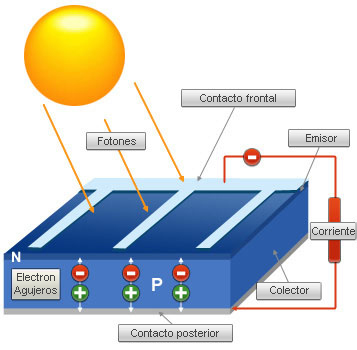
\includegraphics[scale=.50]{Capitulo2/images/celula-fotovoltaica.jpg}
	\caption{Ilustración del Efecto Fotoeléctrico}
	\label{fig:diagrama_dispensador}
\end{figure}

\paragraph{}
Los paneles fotovoltaicos se clasifican en función del tipo de célula que los forman, hay células cristalinas y amorfas, las células cristalinas se dividen de la siguiente forma :

\begin{itemize}
	\item Monocristalinas: se componen de secciones de un único cristal de silicio reconocibles por su forma circular u octogonal.
	\item Policristalinas: cuando están formadas por pequeñas partículas cristalizadas.
\end{itemize}

\begin{figure}[H]
	\centering
	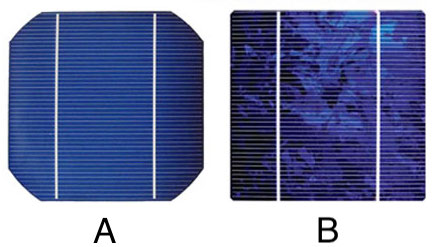
\includegraphics[scale=.50]{Capitulo2/images/tipospaneles.jpg}
	\caption{De izquierda a derecha, célula monocristalina y célula policristalina}
	\label{fig:diagrama_dispensador}
\end{figure}

El costo de los paneles fotovoltaicos se ha reducido de forma constante desde que se fabricaron las primeras células solares comerciales y su coste medio de generación eléctrica ya es competitivo con las fuentes de energía convencionales en un creciente número de regiones geográficas.
Los paneles fotovoltaicos pueden llegar a generar gran cantidad de energía ya que en un día soleado el Sol puede irradiar alrededor de 1kw por metro cuadrado a la superficie de la tierra, que sumado a la eficacia de estos paneles puede llegar a generar entre 120 y 250 w de manera constante por metro cuadrado, siempre dependiendo del tipo de panel y de su nivel de eficiencia.

\paragraph{Módulo Fotovoltaico 250W Policristalino IUSA}
Módulo fotovoltaico con 60 celdas en silicio policristalino, vidrio templado anti reflejante de 3.2 mm, caja de conexión IP67 con 3 diodos bypass y conectores compatibles con MC4.
Tiene una potencia máxima de 250W y un voltaje máximo de 30.6V, con una eficiencia del 15.1 porciento y temperatura de operación entre los -40ºC a los 85ºC. \citep{MarcoTeorico3}.

\begin{figure}[H]
	\centering
	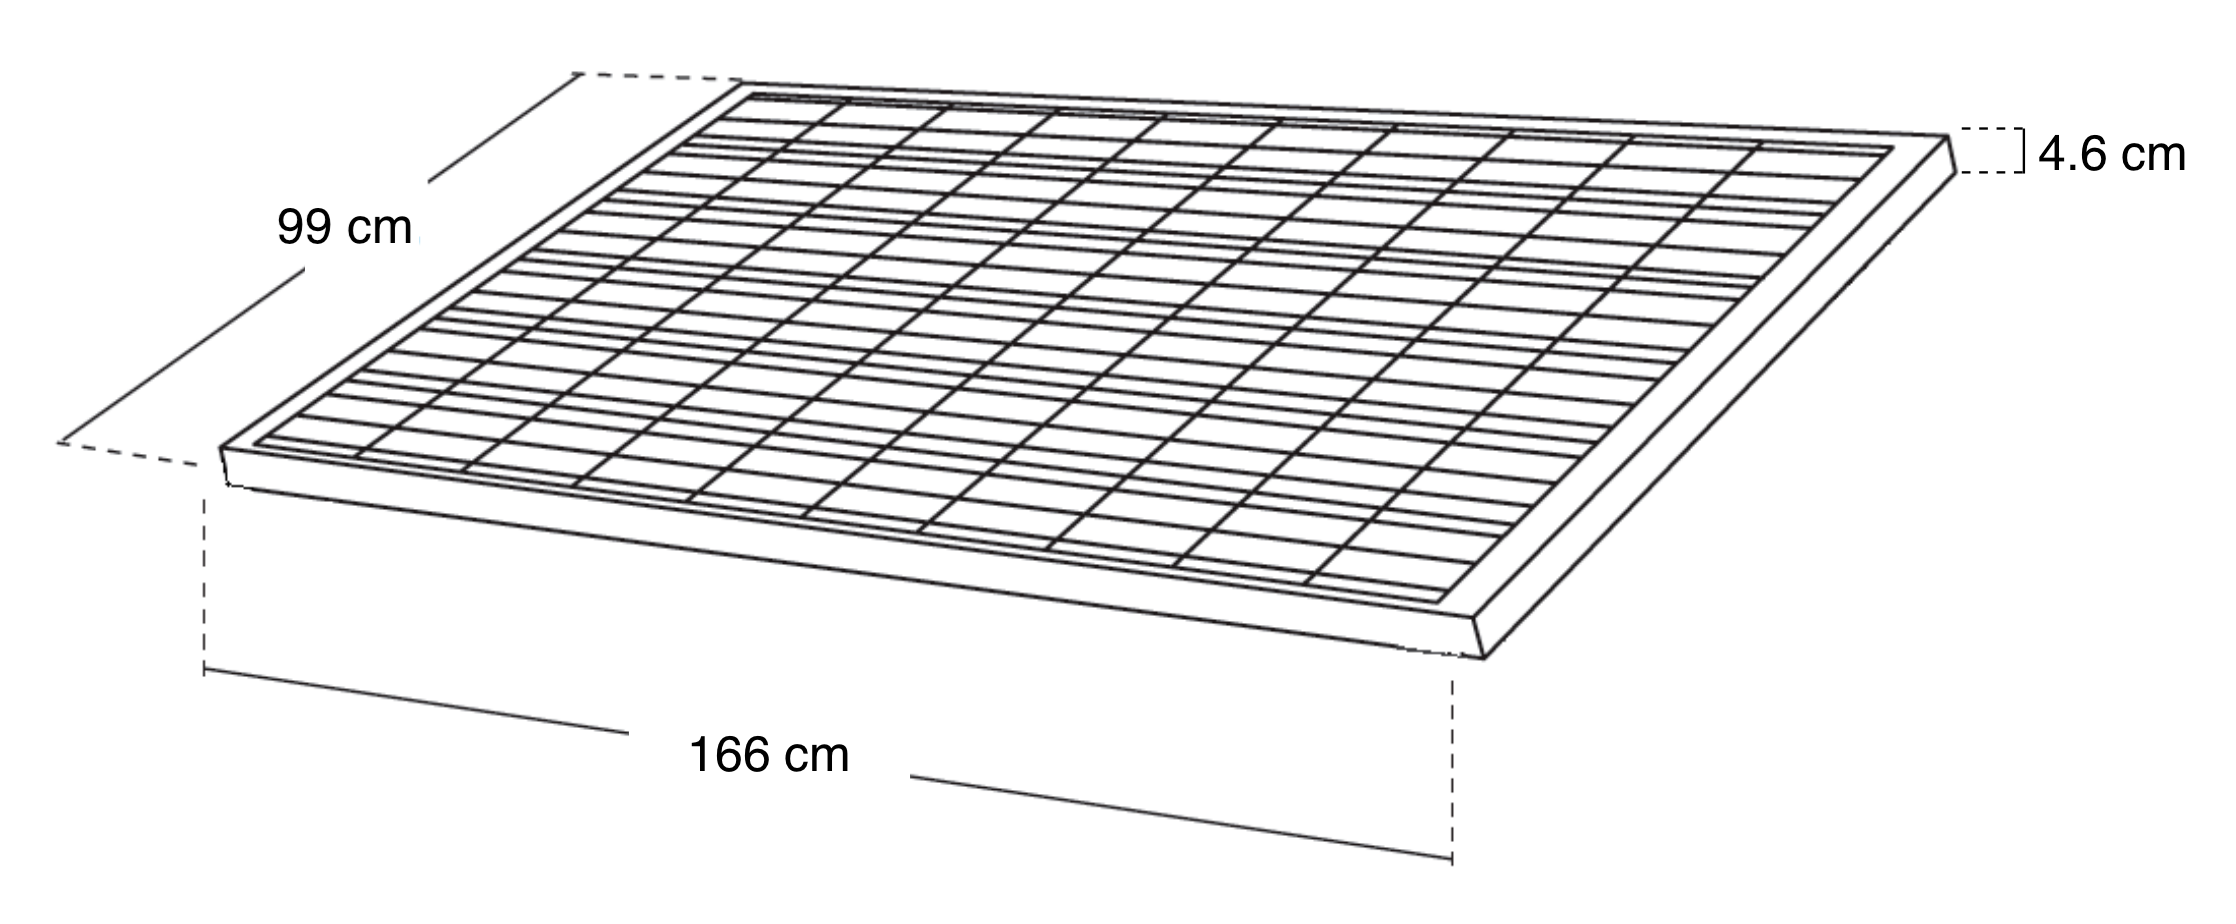
\includegraphics[scale=.25]{Capitulo2/images/panel.png}
	\caption{Esquema del Panel Fotovoltaico, A: 166 cm, B: 99 cm. C: 4.6 cm}
	\label{fig:diagrama_dispensador}
\end{figure}

\paragraph{Microinversor de corriente CC/CA para módulo fotovoltaico M1-01-250}
Diseñado específicamente para interconexiones en el sistema de distribución mexicano, con una salida de 127 V a 60 Hz CA y conector MC4 para conectar el panel solar \citep{MarcoTeorico3}.

\begin{figure}[H]
	\centering
	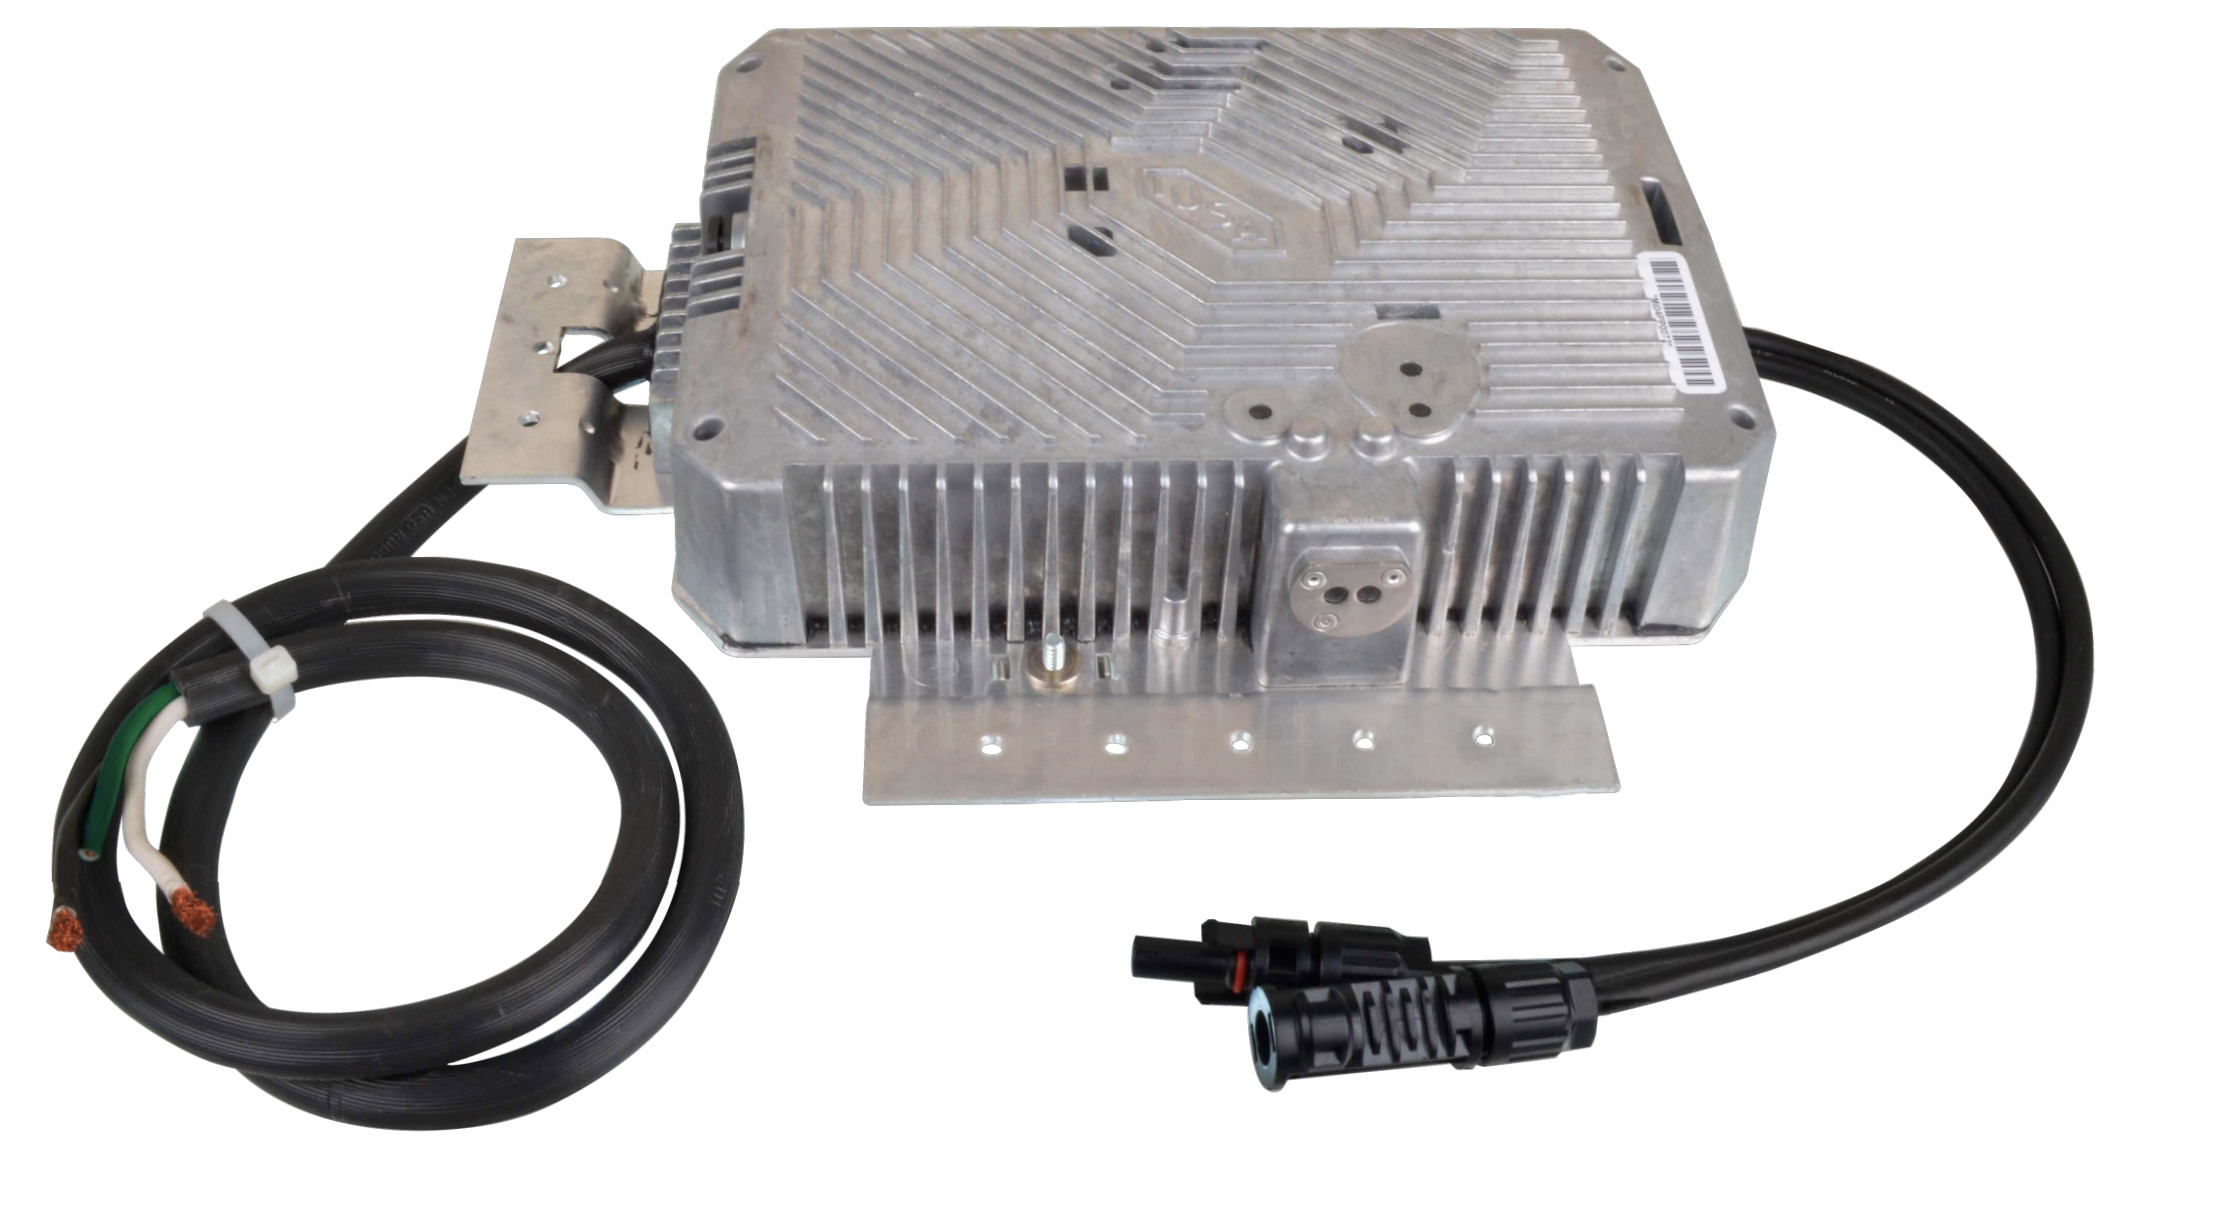
\includegraphics[scale=.25]{Capitulo2/images/microinversor.png}
	\caption{Esquema del Panel Fotovoltaico, A: 166 cm, B: 99 cm. C: 4.6 cm}
	\label{fig:diagrama_dispensador}
\end{figure}
 
\section{MIKROE-2542}

MIKROE-2542 es una placa con un adaptador tipo mikroBUS que integra el modulo ESP-WROOM-02, este último esta compuesto por una antena PCB y el chip ESP8266EX \citep{MarcoTeorico5}.

\begin{figure}[H]
	\centering
	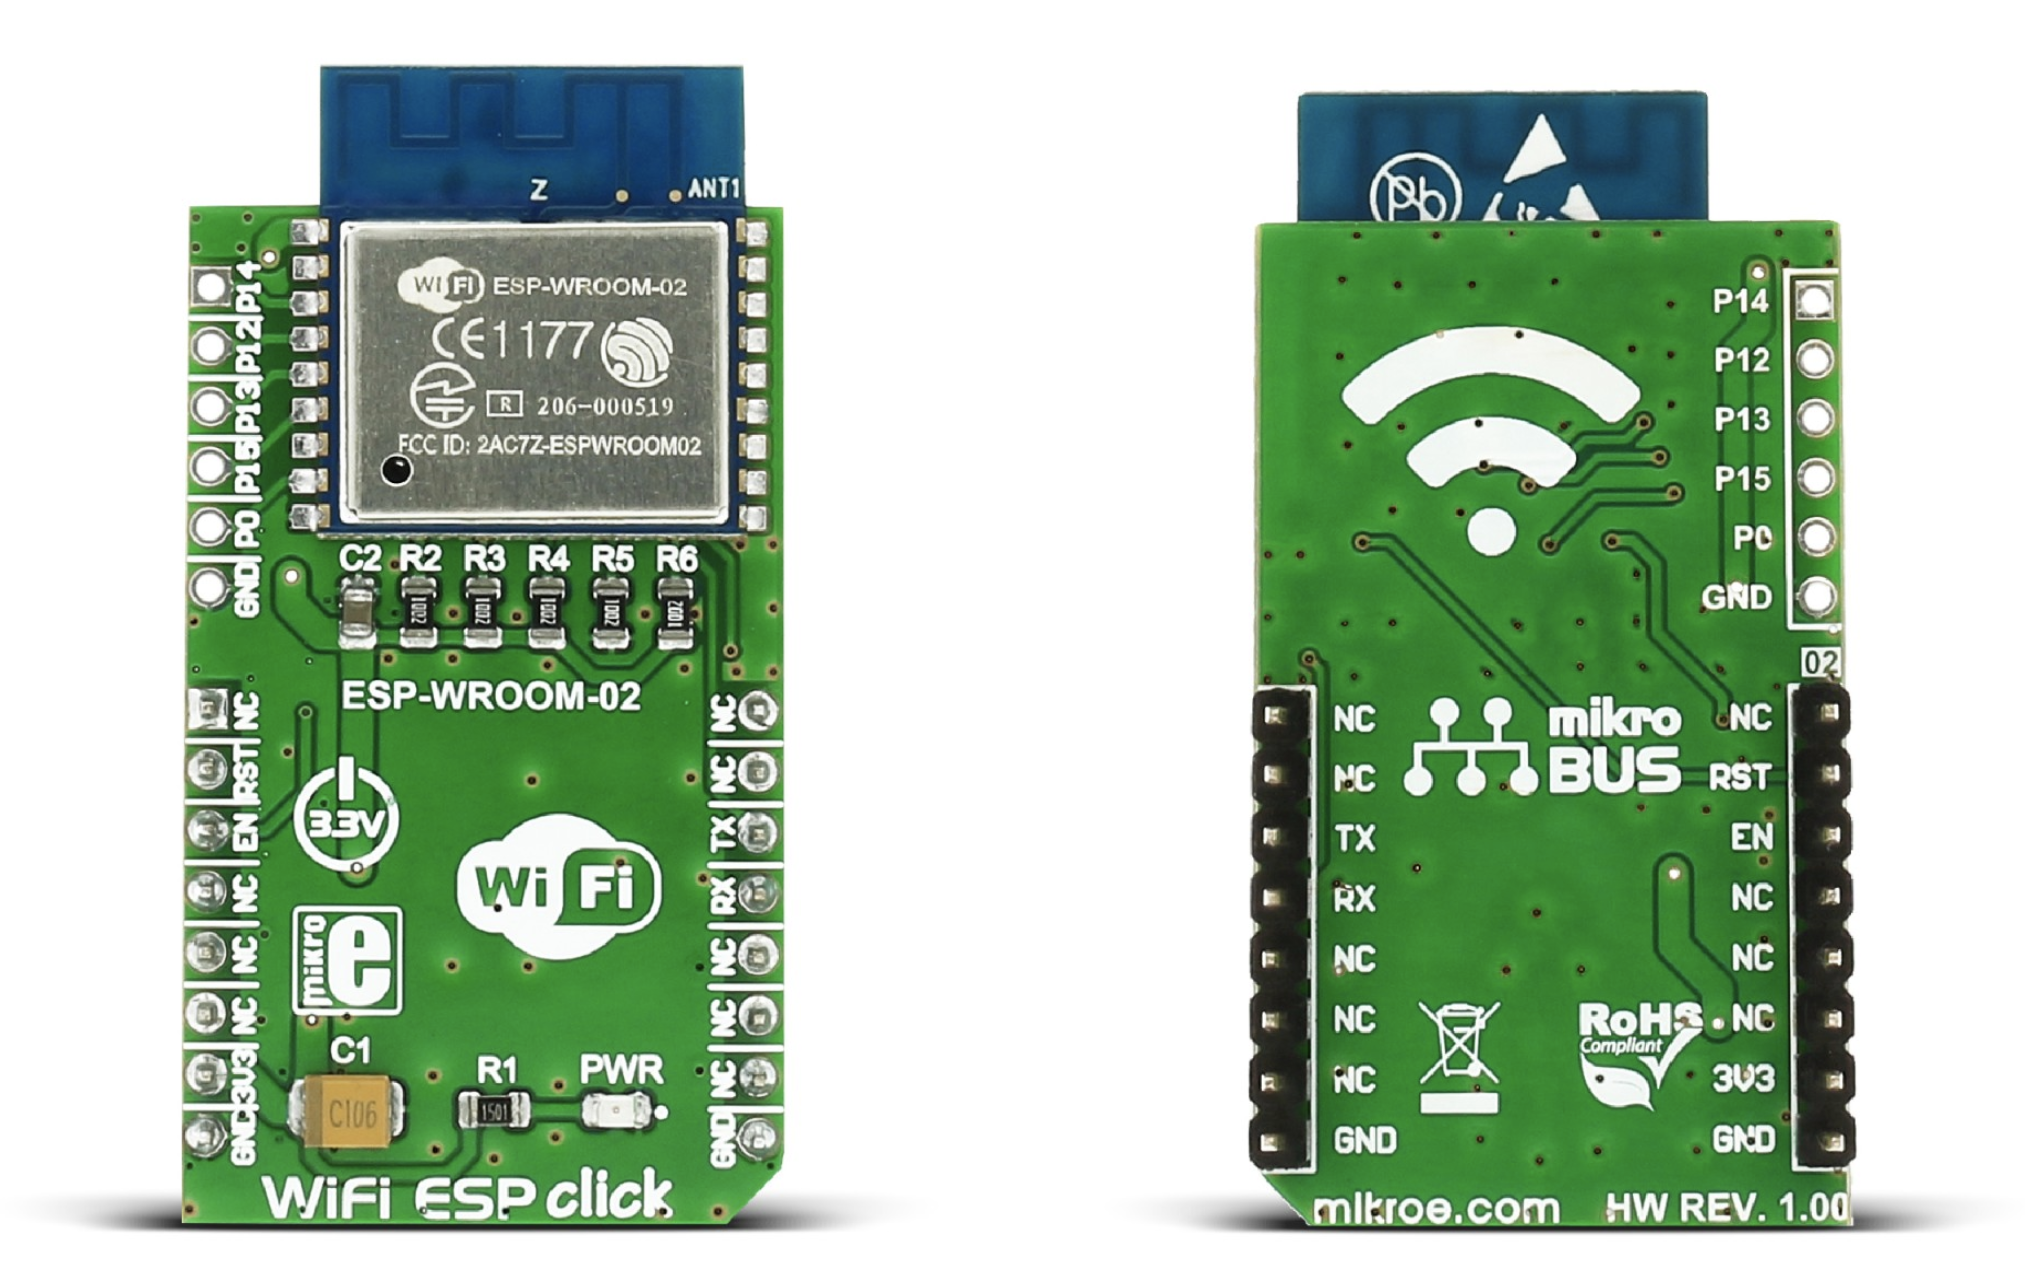
\includegraphics[scale=.25]{Capitulo2/images/mikroe.png}
	\caption{Placa MIKROE-2542}
	\label{fig:diagrama_dispensador}
\end{figure}
\paragraph{}

\begin{figure}[H]
	\centering
	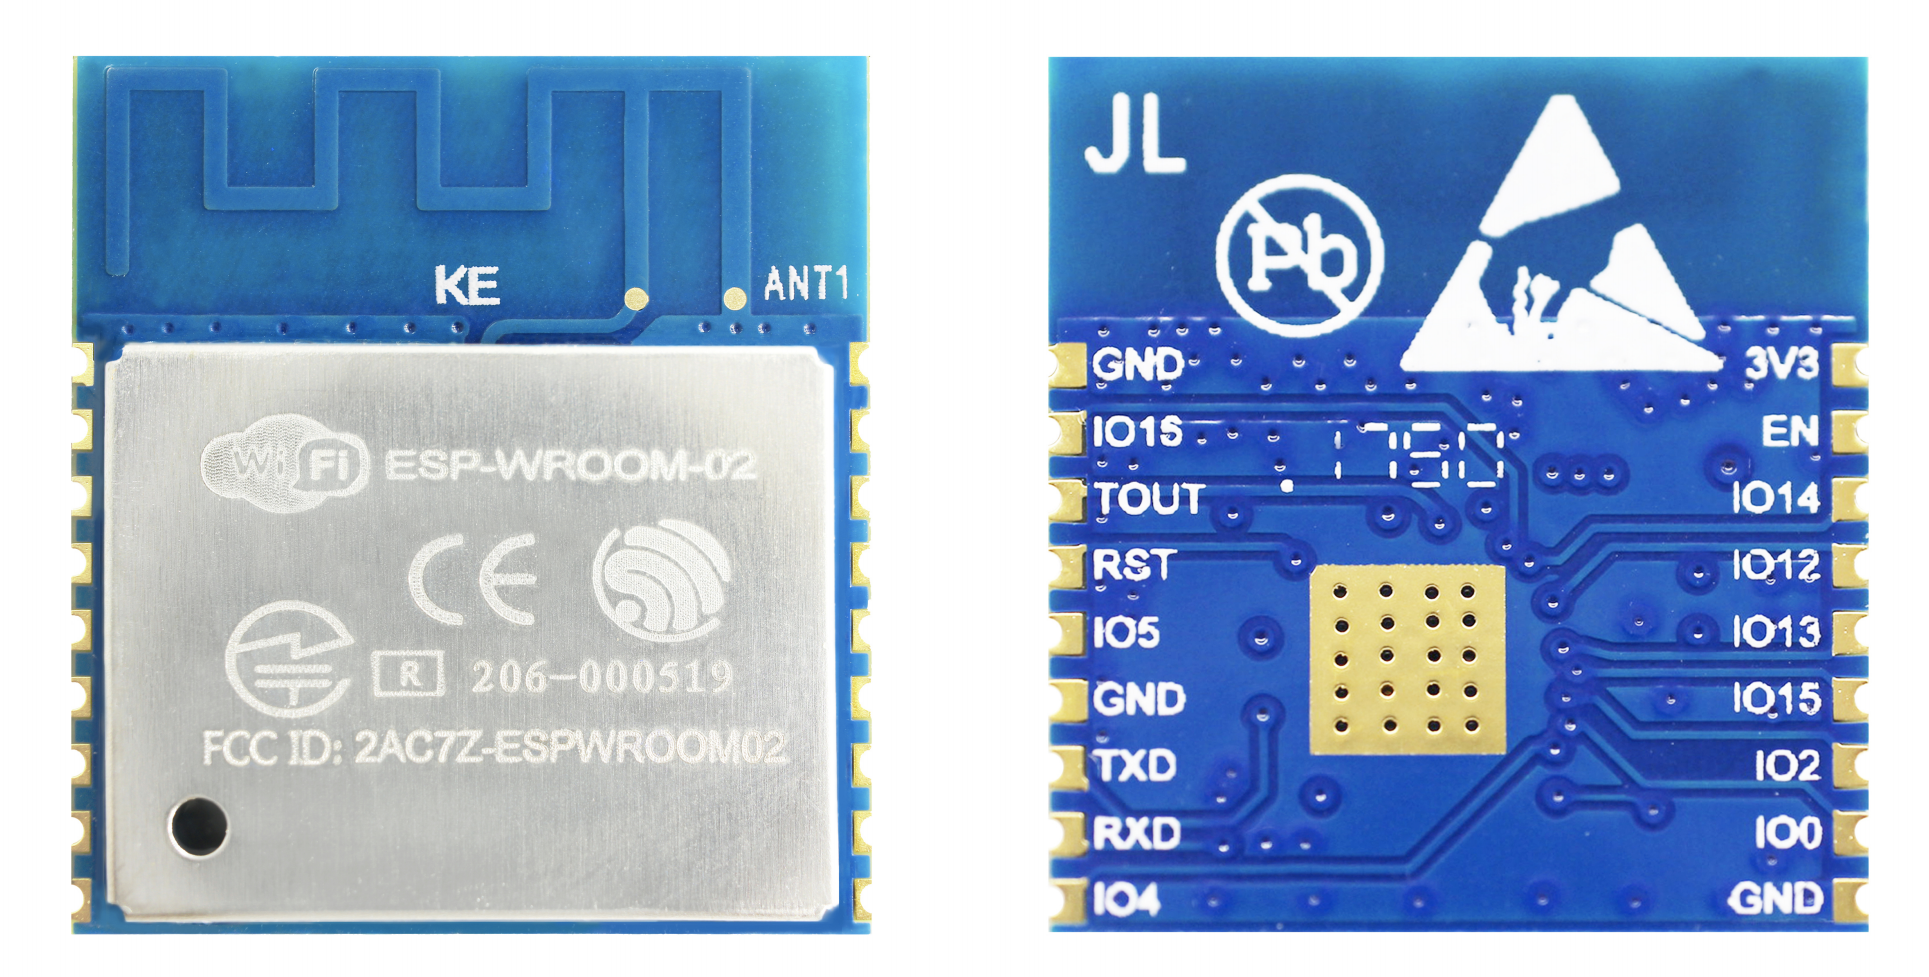
\includegraphics[scale=.25]{Capitulo2/images/wroom.png}
	\caption{Modulo ESP-WROOM-02}
	\label{fig:diagrama_dispensador}
\end{figure}


\paragraph{MikroBUS}
Es un estándar de distribución de los pines para la conexión y comunicación entre un microcontrolador o microprocesador con circuitos integrados o módulos, permitiendo así extender las capacidades de los mismos, este estándar incluye los pines requeridos por las tarjetas de desarrollo más actuales \citep{MarcoTeorico5}.
\begin{figure}[H]
	\centering
	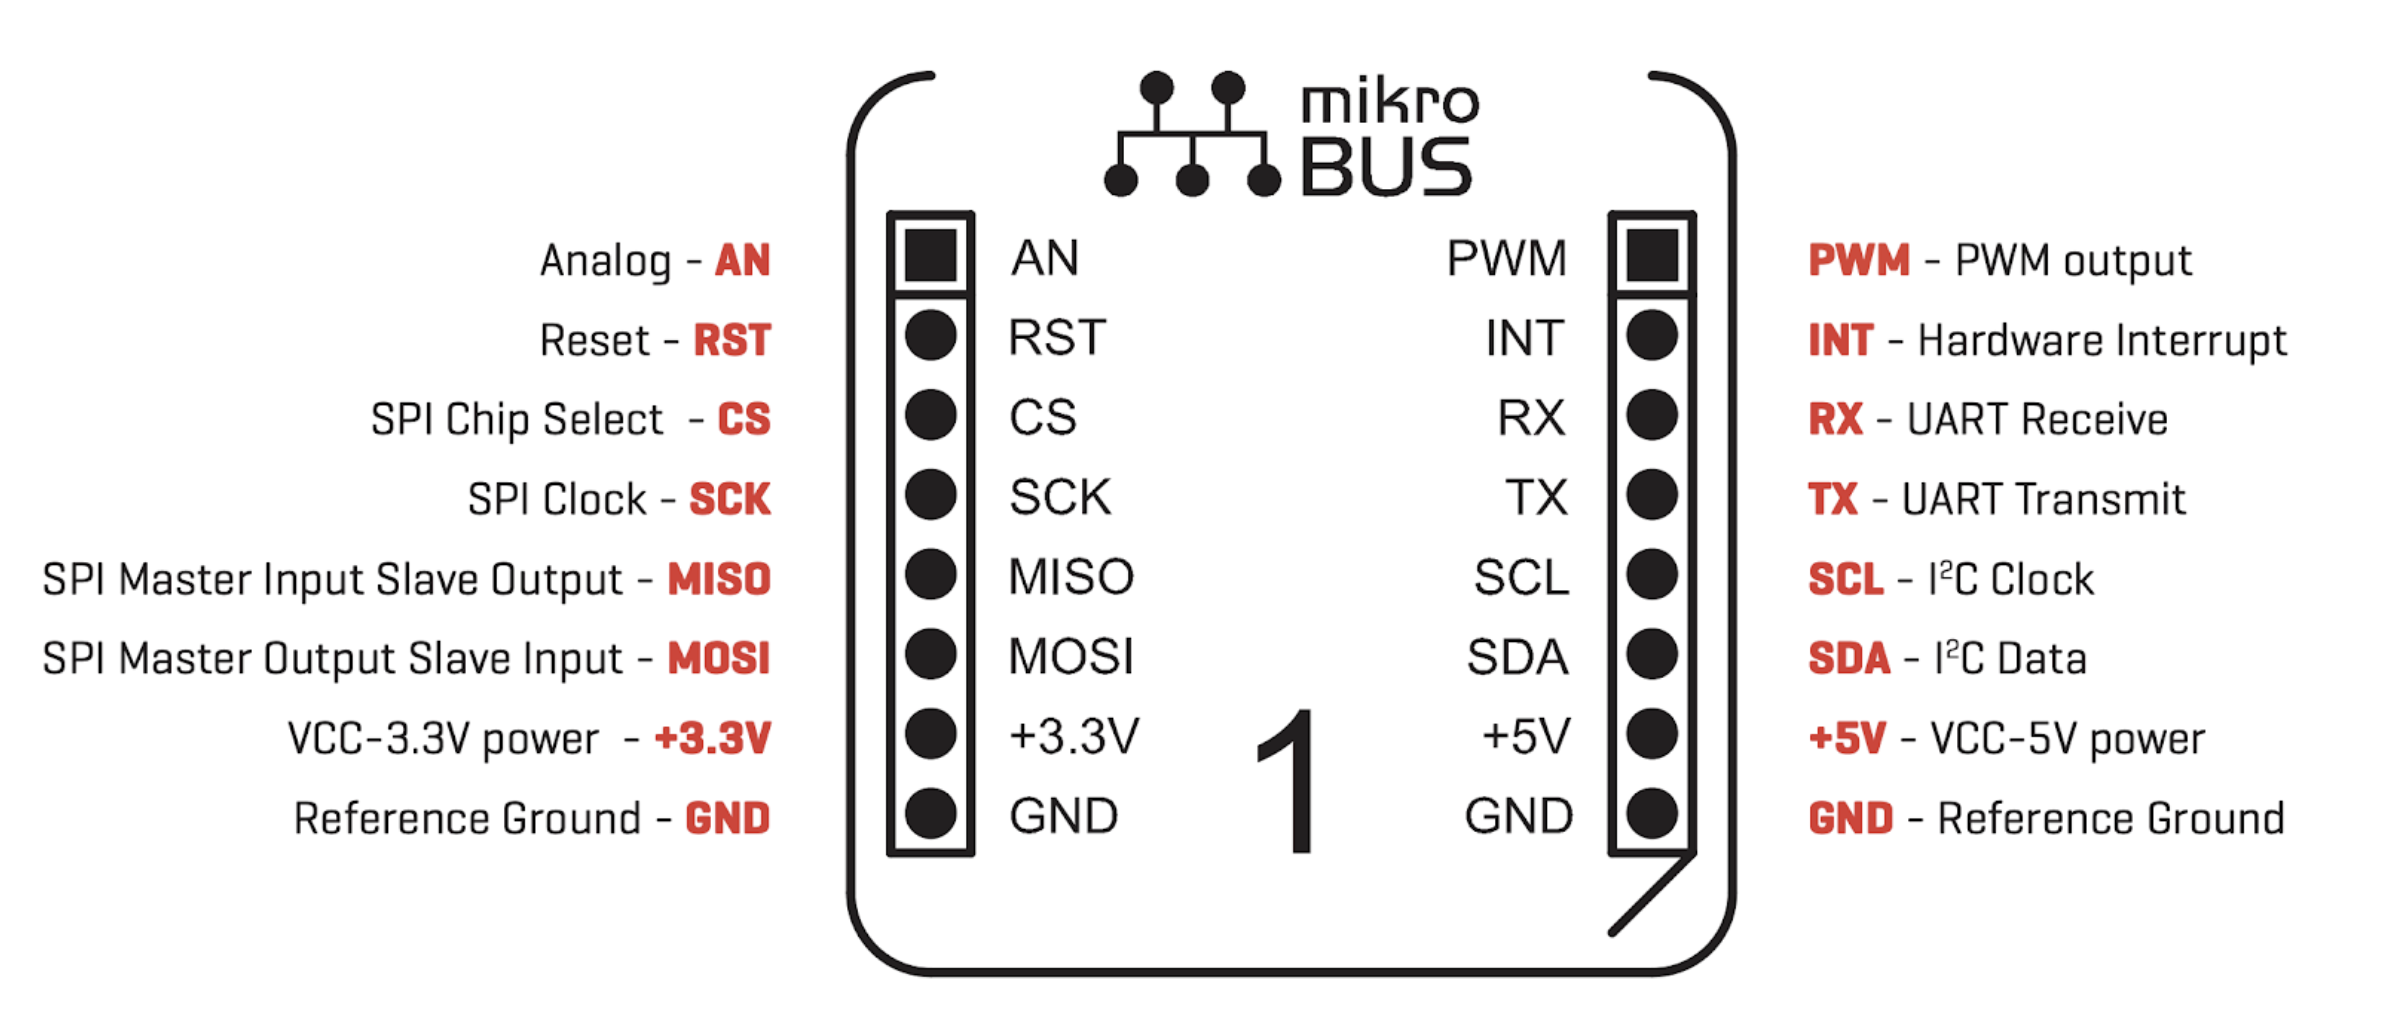
\includegraphics[scale=.25]{Capitulo2/images/mikrobus.png}
	\caption{Distribucion de pines tipo Mikrobus}
	\label{fig:diagrama_dispensador}
\end{figure}
\paragraph{}

\paragraph{ESP8266}
El ESP8266 es un SoC Wi-Fi \citep{MarcoTeorico7} (System on Chip: integra todos o gran parte de los módulos que componen un sistema electrónico en un único circuito integrado) compuesto por una pila TCP/IP y un microcontrolador \citep{MarcoTeorico8}.
\paragraph{}

Este módulo permite a otros microcontroladores conectarse a un red inalámbrica Wi-Fi y realizar conexiones simples con TCP/IP haciendo uso eficiente de energía, lo cual lo hace ideal para proyectos de IoT. A continuación se muestra un a comparativa con otros módulos WiFi, la elección de este modulo es debido a que tiene solamente las características de comunicación de WiFi necesarias y  suficientes para la aplicación a desarrollar, además de un costo promedio:

\begin{figure}[H]
	\centering
	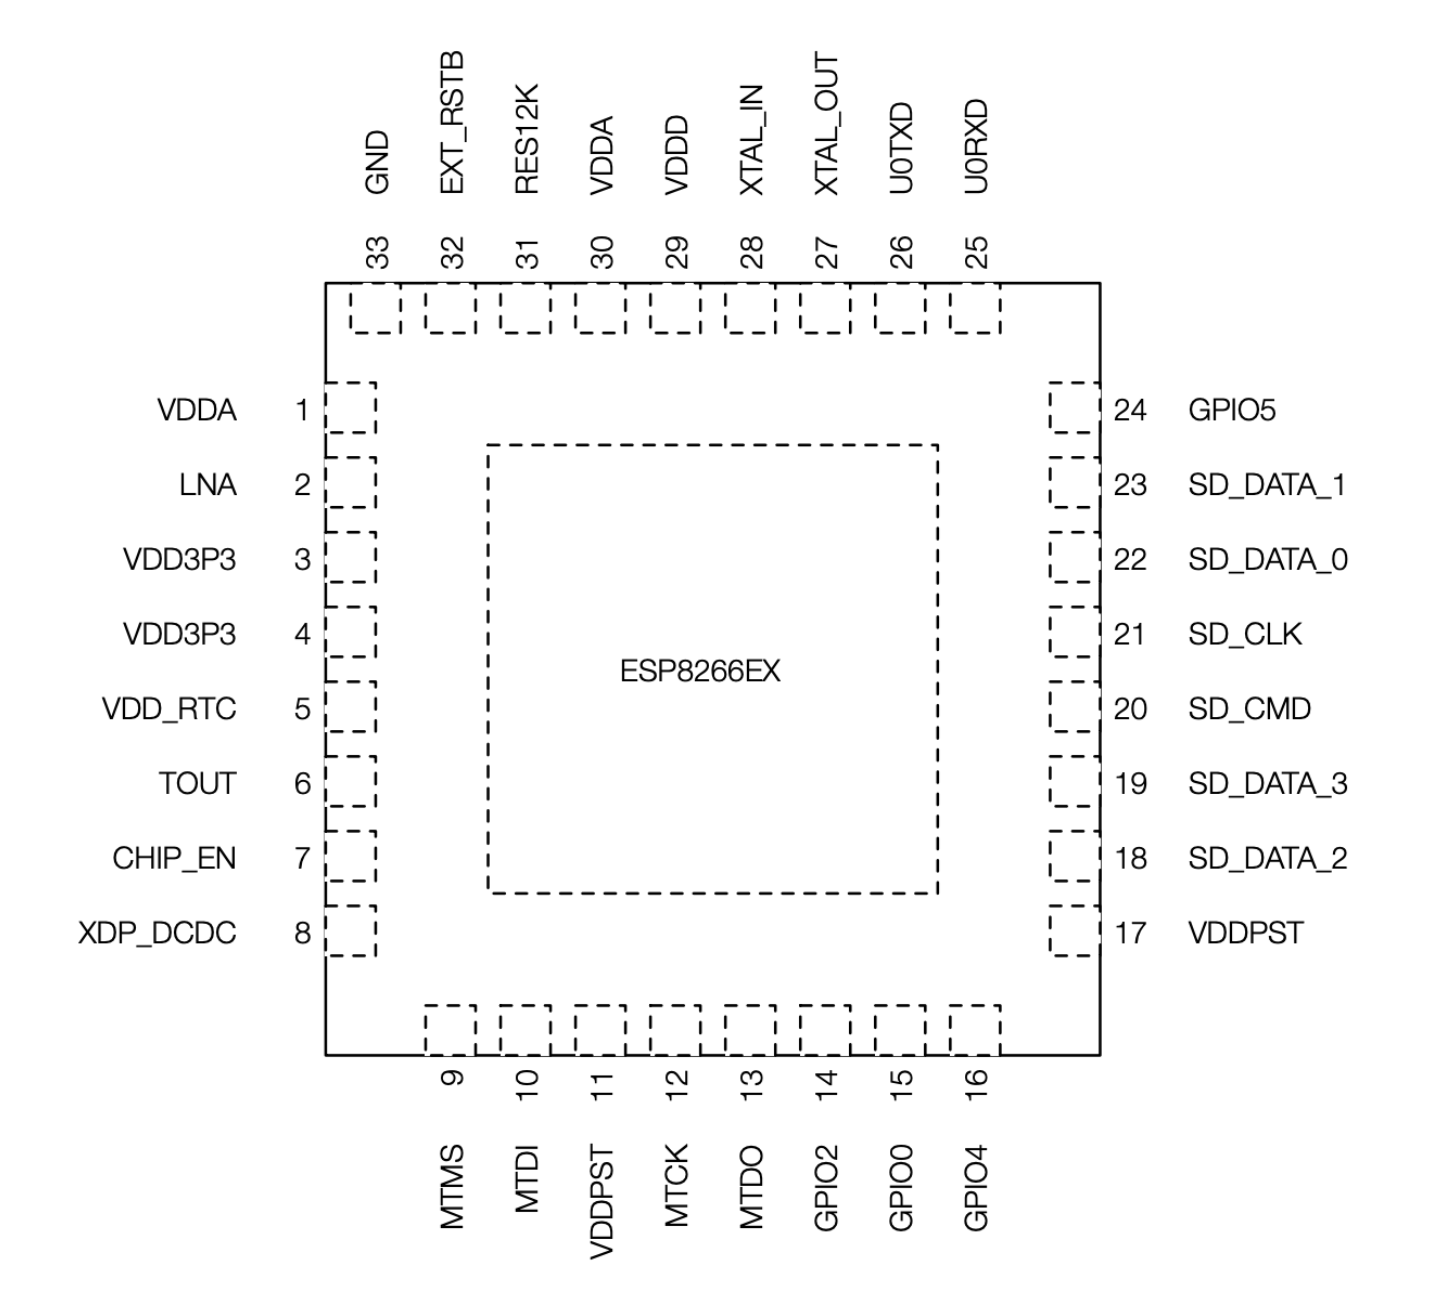
\includegraphics[scale=.25]{Capitulo2/images/esp8266.png}
	\caption{Diagrama esquemático del chip esp8266}
	\label{fig:diagrama_dispensador}
\end{figure}

\pagebreak

\begin{longtable}{|M{2.2cm}|M{4.0cm}|M{4.0cm}|M{4.0cm}|}
	% \centering
	% \begin{tabular}
	\hline
	\textbf{Categoría} & \textbf{MIKROE-2542} & \textbf{356-ESP32-PICO-KIT} & \textbf{GPy 1.0} \\ \hline
	
 	Fabricante & MikroElektronika & Espressif Systems & Pycom
 	\hline
 	 
    Wi-Fi 
    &
    \newline  -Protocolo estándar IEEE 802.11
    \newline  -Rango de frecuencia 2.4G ~ 2.5G 
    \newline  -Antena PCB
	& 
    \newline  -Protoloco estándar IEEE 802.11
    \newline  -Rango de frecuencia 2.4G ~ 2.5G 
    \newline  -Antena 3D
	&   	    
    \newline  -Protoloco estándar IEEE 802.11
    \newline  -Rango de frecuencia 2.4G ~ 2.5G 
    \newline  -Antena Bluetooth y WiFi interna
    \newline  -Conector para antena LTE CAT M1 / NB1
    \newline  -Transceiver LTE CAT M1/ NB1 	
    \hline

	Bluetooth 
    &
	---
    &
	\newline Protocolo Bluetooth V4.2
	&
	\newline Protocolo Bluetooth V4.2 
	\hline
	
	Hardware &
    \newline  -CPU Tensilica L106 32-bit processor
    \newline  -Interfaz Periférica UART/SDIO/SPI/I2C/I2S/IR Control Remoto
    \newline  -Intefaces GPIO/ADC/PWM/LED Light
    \newline  -Voltaje de operación entre 2.5V ~ 3.6V
    &
    \newline  -CPU ESP32-PICO-D4
    \newline  -Interfaz Periférica ADC, DAC, sensor touch, SD/SDIO/MMC Host Controller, SPI, SDIO/SPI Controlador Esclavo, EMAC, motor PWM, LED PWM, UART, I2C, I2S, Control Remoto Infrarojo 
    \newline  -Voltaje de operación entre 2.5V ~ 3.6V
    \newline  -Sensor Hall integrado
    \newline  -Cristal de 40 MHz
    \newline  -SPI flash de 4MB integrada
    &
    \newline  - CPU Espressif ESP32 SoC
    \newline  - Coprocesador ULP
    \newline  - Interfaz Periférica ADC Controller
    \newline  - Voltaje de operación entre 2.5V ~ 3.6V
    \newline  - Memoria flash de 8MB integrada
    &
	\hline
	
    Precio (USD) & \$ 19.50 & \$ 13.00 & \$ 71.40
    \hline
	
	% \end{tabular}
	\caption{Comparativa con otros módulos WiFi}
	\label{tabla_riesgos}
\end{longtable}

\pagebreak

\section{Demonio / Servicio}
Un demonio o servicio es un programa que se ejecuta en segundo plano, fuera del control interactivo de los usuarios del sistema ya que carecen de interfaz con estos. El término demonio se usa fundamentalmente en sistemas UNIX y basados en UNIX, como GNU/Linux o Mac OS X \citep{MarcoTeorico4}.

\section{Dispositivo de monitoreo de energía}
En este trabajo se plantea el uso de un dispositivo de monitoreo de energía que permita supervisar de manera constante la energía producida por las celdas fotovoltaicas; es por ello que a continuación definiremos algunos conceptos importantes.
\paragraph{}
Inicialmente, un dispositivo puede ser definido como un mecanismo dispuesto para obtener un resultado automático\citep{MarcoTeorico11}; es decir, un conjunto de elementos bien definidos, que entre sí, realizan acciones conforme la información recibida (entrada) para poder transformarla (salida).
Existe una amplia gama de clasificación de dispositivos de acuerdo al propósito para el que es empleado, sin embargo, para fines de este trabajo, el dispositivo de interés entra en la categoría de aquellos que se encargan de monitorear. 
\paragraph{}
De acuerdo a la Real Academia Española, la palabra monitorear, se define como la acción de observar, supervisar o controlar mediante aparatos especiales, el curso de uno o varios parámetros fisiológicos o de otra naturaleza para detectar posibles anomalías.\citep{MarcoTeorico12}
\paragraph{}
Teniendo en cuenta los 2 conceptos anteriores, podemos definir a un dispositivo de monitoreo de energía como: un mecanismo que recibe como entrada energía e internamente procesa dicha información para finalmente arrojar datos de monitoreo.
\paragraph{}
El dispositivo que se usará es el MCP39F521 (I2C Power Monitor with Calculation and Energy Accumulation), el cual se define como un dispositivo de alta integración de monitoreo de energía de fase completa, diseñado para realizar medición en tiempo real de la energía de entrada para las fuentes de alimentación de corriente directa o alterna, unidades de distribución de energía y aplicaciones de consumidor e industriales.\citep{MarcoTeorico13}
\paragraph{}
\begin{figure}[H]
	\centering
	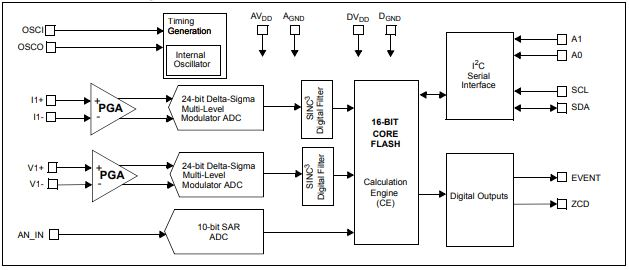
\includegraphics[scale=.9]{Capitulo2/images/DiagramaDispMonitoreo.JPG}
	\caption{Diagrama a bloques del MCP39F521}
	\label{fig:diagrama_dispMonitoreo}
\end{figure}


\section{Sistema Embebido}
Un sistema embebido es un dispositivo diseñado para un propósito en específico, el cual puede abarcar desde una operación hasta un conjunto pequeño de operaciones en tiempo real, a diferencia de una PC, la cual puede realizar una gran cantidad de tareas de acuerdo a los programas que se ejecuten. 
\paragraph{}
El uso de los sistemas embebidos ha cobrado gran importancia debido a los usos y aplicaciones que se le han dado, como son: hornos de microondas, máquinas expendedoras, routers, cámaras digitales, reproductores MP3, entre otros. 
\paragraph{}
Algunas de las características principales de los sistemas embebidos son: que tienden a ser de dimensiones pequeñas, son considerados económicos o de bajo costo, su nivel de consumo eléctrico es bajo, poseen recursos limitados de memoria así como de dispositivos de entrada/salida.\citep{MarcoTeorico14}
\paragraph{}
Por lo general, los sistemas embebidos al ofrecer como ventaja la realización de operaciones en tiempo real, suelen ser empleados en ambientes físicos donde se hace uso de sensores y actuadores. Se dice que son sistemas reactivos, pues están en interacción continua con su entorno y el ritmo de su ejecución está coordinada con dicho entorno. 
\paragraph{}
Los sistemas embebidos suelen tener en una de sus partes una computadora con características especiales conocida como microcontrolador que viene a ser el cerebro del sistema, el cual incluye interfaces de entrada/salida en el mismo chip. Normalmente estos sistemas poseen un interfaz externo para efectuar un monitoreo del estado y hacer un diagnóstico del sistema.\citep{MarcoTeorico15}
\paragraph{}
Los sistemas embebidos se encuentran implementados en placas únicas (SBC como una Raspberry) y sobre estas se encuentran integrados los recursos de hardware como el microprocesador, la memoria RAM, controladores ethernet, etc.\citep{MarcoTeorico14}

\section{Red de sensores}
Una red de sensores consiste en un conjunto de dispositivos denominados sensores que están conectados entre sí, para el monitoreo y sensado de condiciones físicas y/o ambientales en áreas remotas; dichos sensores pueden estar distribuidos físicamente y para referirnos a un sensor en específico como parte de la red, se le denomina nodo sensor. 
\paragraph{}
El propósito de una red de sensores es el de recolectar información de interés, es decir, la variable física sensada o monitoreada, para posteriormente transmitir dicha información con el objeto de ser procesada y analizada. 
\paragraph{}
Dado que existen una gran cantidad de dispositivos sensores implica que pueden implementarse diferentes tipos de redes de sensores de acuerdo al uso o aplicación que se le quiera dar, como por ejemplo: fenómenos meteorológicos, sistemas de emergencia o de cuidados médicos, por mencionar algunos.\citep{MarcoTeorico16}